\documentclass[]{article}

\usepackage[utf8]{inputenc}
\usepackage{neuralnetwork}
\usepackage{todonotes}
\usepackage{hyperref}
\usepackage{pbox}
\usepackage{tabularx}
\usepackage{lscape}

\title{Introduction to Intelligent Systems \\ Project2: Recycling used parts for fun and profit}
\author{Joseph Fuchs, Damien Crémilleux}

\begin{document}

\maketitle

\section{Classifier Design}
To solve this classification problem, we use two different techniques:
\begin{itemize}
\item Multi-layer perceptron
\item Decision tree ensemble
\end{itemize}

The multi-layer perceptron has two input nodes, five hidden nodes, and four output nodes (for four classes), plus bias nodes (a 2-5-4 architecture), as suggested in the wording. This multi-layer perceptron is illustrated in Figure~\ref{fig:neural_network} page~\pageref{fig:neural_network}. The bias node are in yellow.
\begin{figure}
  \centering
  \begin{neuralnetwork}[height=2.5, layertitleheight=0, nodespacing=2cm, layerspacing=2cm]
    \newcommand{\nodetextclear}[2]{}
    \newcommand{\nodetextxnb}[2]{\ifnum0=#2 \else $x_#2$ \fi}
    \newcommand{\nodetexth}[2]{$0.5$}
    \newcommand{\nodetextO}[2]{$output$}
    \newcommand{\logiclabel}[1]{\,{$\scriptstyle#1$}\,}
    \newcommand{\nodetextY}[2]{$0.5$}
    \newcommand{\linklabelsU}[4]{\logiclabel{+1}}
    \newcommand{\linklabelsV}[4]{\logiclabel{-1}}
    \newcommand{\linklabelsA}[4]{\ifnum0=#2 \logiclabel{+3} \else \logiclabel{-2} \fi}
    \setdefaultnodetext{\nodetextclear}

    % data layer
    \datalayer[count=2, bias=false, text=\nodetextxnb]

    % links to data layer to input layer
    \inputlayer[count=2, bias=true]
    \link[from layer=0, to layer=1, from node=1, to node=1]
    \link[from layer=0, to layer=1, from node=2, to node=2]

    % links to hidden layer from input layer
    \hiddenlayer[count=5, bias=true]
    \link[from layer=1, to layer=2, from node=0, to node=1]
    \link[from layer=1, to layer=2, from node=0, to node=2]
    \link[from layer=1, to layer=2, from node=0, to node=3]
    \link[from layer=1, to layer=2, from node=0, to node=4]
    \link[from layer=1, to layer=2, from node=0, to node=5]

    \link[from layer=1, to layer=2, from node=1, to node=1]
    \link[from layer=1, to layer=2, from node=1, to node=2]
    \link[from layer=1, to layer=2, from node=1, to node=3]
    \link[from layer=1, to layer=2, from node=1, to node=4]
    \link[from layer=1, to layer=2, from node=1, to node=5]

    \link[from layer=1, to layer=2, from node=2, to node=1]
    \link[from layer=1, to layer=2, from node=2, to node=2]
    \link[from layer=1, to layer=2, from node=2, to node=3]
    \link[from layer=1, to layer=2, from node=2, to node=4]
    \link[from layer=1, to layer=2, from node=2, to node=5]
    
    \outputlayer[count=4, bias=false]
    % links to output layer from second hidden layer
    \link[from layer=2, to layer=3, from node=0, to node=1]
    \link[from layer=2, to layer=3, from node=0, to node=2]
    \link[from layer=2, to layer=3, from node=0, to node=3]
    \link[from layer=2, to layer=3, from node=0, to node=4]

    \link[from layer=2, to layer=3, from node=1, to node=1]
    \link[from layer=2, to layer=3, from node=1, to node=2]
    \link[from layer=2, to layer=3, from node=1, to node=3]
    \link[from layer=2, to layer=3, from node=1, to node=4]

    \link[from layer=2, to layer=3, from node=2, to node=1]
    \link[from layer=2, to layer=3, from node=2, to node=2]
    \link[from layer=2, to layer=3, from node=2, to node=3]
    \link[from layer=2, to layer=3, from node=2, to node=4]

    \link[from layer=2, to layer=3, from node=3, to node=1]
    \link[from layer=2, to layer=3, from node=3, to node=2]
    \link[from layer=2, to layer=3, from node=3, to node=3]
    \link[from layer=2, to layer=3, from node=3, to node=4]

    
    \link[from layer=2, to layer=3, from node=4, to node=1]
    \link[from layer=2, to layer=3, from node=4, to node=2]
    \link[from layer=2, to layer=3, from node=4, to node=3]
    \link[from layer=2, to layer=3, from node=4, to node=4]
    
    \link[from layer=2, to layer=3, from node=5, to node=1]
    \link[from layer=2, to layer=3, from node=5, to node=2]
    \link[from layer=2, to layer=3, from node=5, to node=3]
    \link[from layer=2, to layer=3, from node=5, to node=4]
    
    % Input data
    \olayer[count=1, bias=false, text=\nodetextO]
    \link[from layer=3, to layer=4, from node=1, to node=1]
    \link[from layer=3, to layer=4, from node=2, to node=1]
    \link[from layer=3, to layer=4, from node=3, to node=1]
    \link[from layer=3, to layer=4, from node=4, to node=1]
  \end{neuralnetwork}
  
  \caption{The architecture of the neural network used to solve this problem}
  \label{fig:neural_network}
\end{figure}

\todo{Illustrate the decision tree}

Decision tree ensemble and neural network are two methods of supervised learning.
This means that each samples of the training data is a pair of an input object (in our case the value for the six-fold rotational symmetry and the eccentricity) and a desired output value (in our case, the class, bolt, nut, ring, scrap).
However neural networks are not easily understandable. Neural networks are like a black box, we can not easily explain how decisions are made. On the contrary, it is easier to see how decisions are made in a decision tree ensemble because we can look at the trees and see how variables divide the data.

\medskip

We expect the multi-layer perceptron to perform better. Several scientific articles\footnote{An example in bio-informatic: \url{http://www.csee.usf.edu/~rbanfiel/papers/NNvsDT.pdf}} show that neural networks have better results than decision tree ensemble. However, the result heavily depends of the input data, this is not always the case.


\section{Data sets}

The training data set is shown in Figure~\ref{fig:train_data} and the test data set is shown in Figure~\ref{fig:test_data}.

\begin{figure}[h]
    \centering
    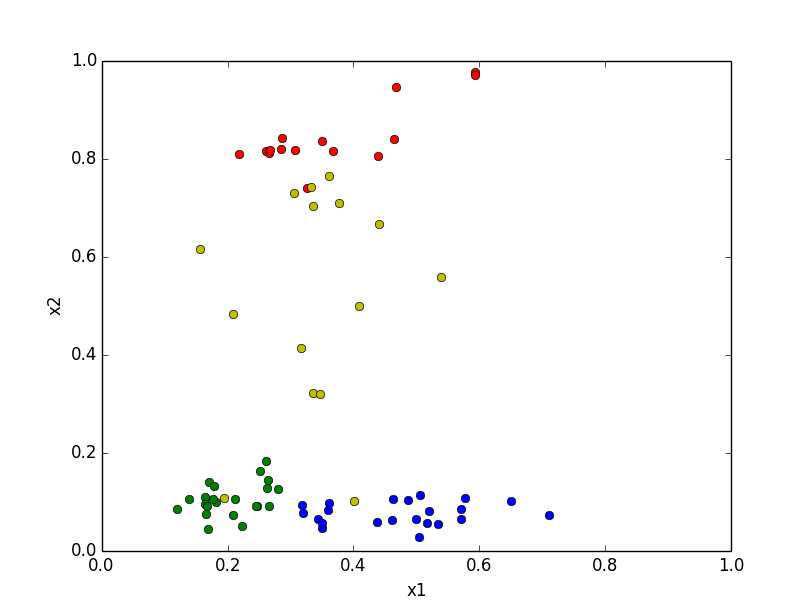
\includegraphics[width=0.9\textwidth]{figures/train_data.png}
    \caption{Training data set}
    \label{fig:train_data}
\end{figure}

\begin{figure}[h]
    \centering
    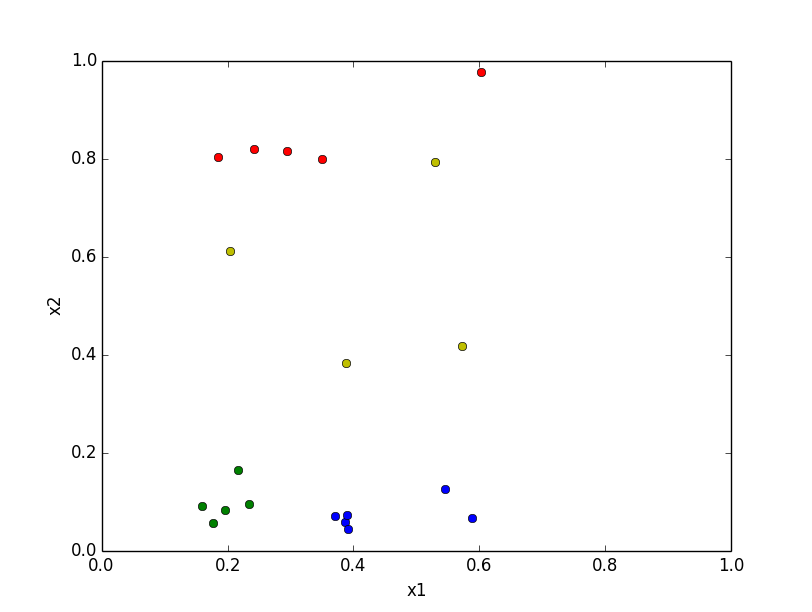
\includegraphics[width=0.9\textwidth]{figures/test_data.png}
    \caption{Test data set}
    \label{fig:test_data}
\end{figure}

The red dots are bolts, the blue dots are nuts, the green dots are rings and the yellow ones are scraps.
We can see that on the test set, the dots are not mixed. This is not the case for the training data set.
A bolt is mixed with scrapds, and scraps are mixed with nuts and rings.
This will lead to some errors of classification for the training data set, but because the different classes are not mixed in the test data set, we can hope that the final classifier will be efficient.

\section{Results}
\label{sec:results}

\subsection{Multi-layer perceptron}

\begin{center}
    \begin{tabularx}{\textwidth}{ | X | X | X | X | X | X | }
    \hline
    Epoch & 0 & 10 & 100 & 1000 & 10000 \\ \hline
    Recognition rate & 0.2 & 0.25 & 0.65 & 1 & 1 \\ \hline
    Profit & -0.6 & -0.8  & 1.03 & 2.03 & 2.03 \\ \hline
    Confusion matrix  & [0, 0, 0, 0] \newline [0, 0, 0, 0] \newline [0, 0, 0, 0] \newline [5, 6, 5, 4] & [0, 0, 0, 0] \newline [0, 0, 0, 0] \newline [5, 6, 5, 4] \newline [0, 0, 0, 0] & [5, 0, 0, 2] \newline [0, 2, 0, 1] \newline [0, 4, 5, 0] \newline [0, 0, 0, 1] & [5, 0, 0, 0] \newline [0, 6, 0, 0] \newline [0, 0, 5, 0] \newline [0, 0, 0, 4] & [5, 0, 0, 0] \newline [0, 6, 0, 0] \newline [0, 0, 5, 0] \newline [0, 0, 0, 4] \\
    \hline
    \end{tabularx}
\end{center}

\subsection{Decision tree ensemble}

\begin{center}
    \begin{tabularx}{\textwidth}{ | X | X | X | X | X | X | }
    \hline
    Epoch & 0 & 10 & 100 & 1000 & 10000 \\ \hline
    Recognition rate & &  &  & &  \\ \hline
    Profit &  &   &  & & \\ \hline
    Confusion matrix  &  &  & & & \\
    \hline
    \end{tabularx}
\end{center}
\todo{complete}

\subsection{Classification regions}

The evolution of the classification regions produced by the multi-layer perceptron is shown from Figure~\ref{fig:mlp_classification_0} to Figure~\ref{fig:mlp_classification_10000}.

\begin{figure}[h]
    \centering
    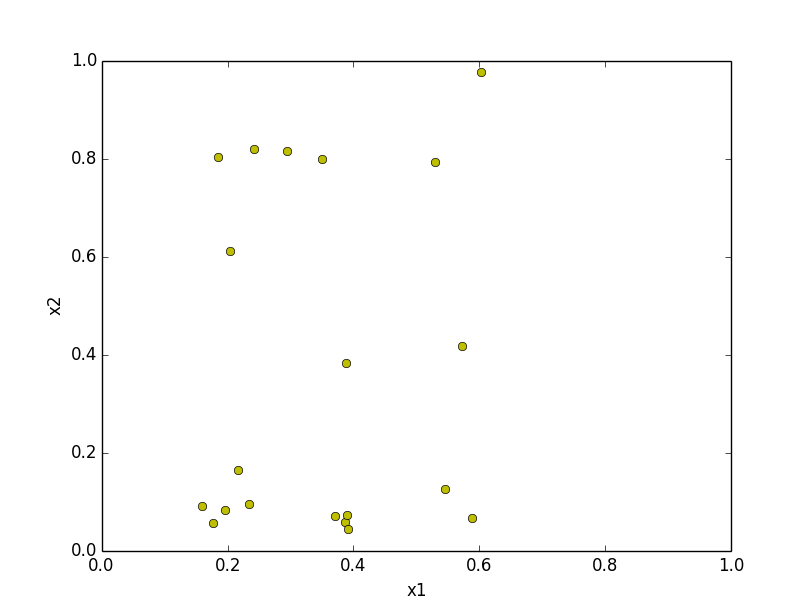
\includegraphics[width=0.9\textwidth]{figures/mlp_classification_0.png}
    \caption{Classification produced by the multi-layer perceptron after 0 epoch}
    \label{fig:mlp_classification_0}
\end{figure}

\begin{figure}[h]
    \centering
    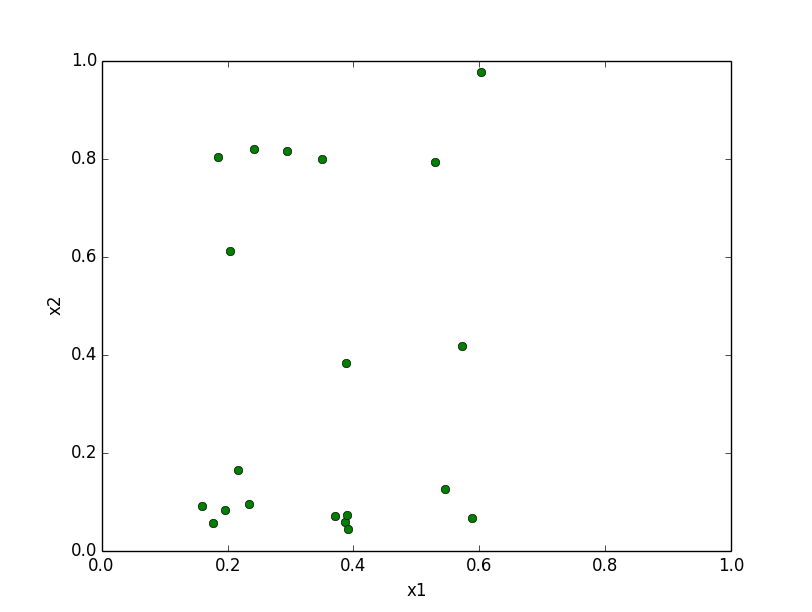
\includegraphics[width=0.9\textwidth]{figures/mlp_classification_10.png}
    \caption{Classification produced by the multi-layer perceptron after 10 epochs}
    \label{fig:mlp_classification_10}
\end{figure}

\begin{figure}[h]
    \centering
    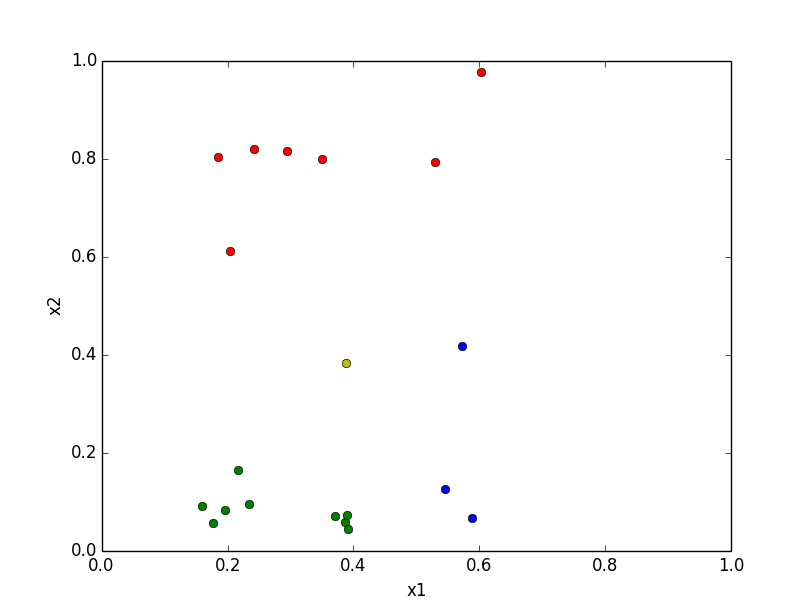
\includegraphics[width=0.9\textwidth]{figures/mlp_classification_100.png}
    \caption{Classification produced by the multi-layer perceptron after 100 epochs}
    \label{fig:mlp_classification_100}
\end{figure}

\begin{figure}[h]
    \centering
    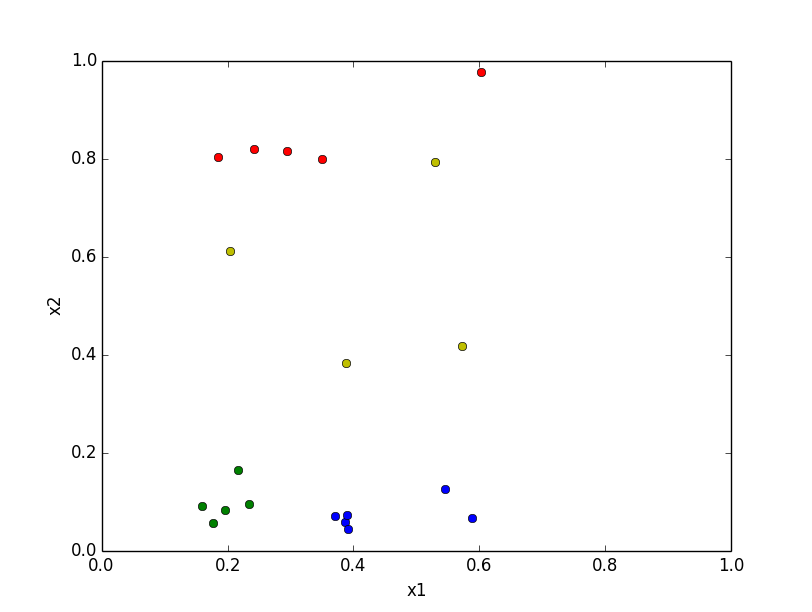
\includegraphics[width=0.9\textwidth]{figures/mlp_classification_1000.png}
    \caption{Classification produced by the multi-layer perceptron after 1000 epochs}
    \label{fig:mlp_classification_1000}
\end{figure}

\begin{figure}[h]
    \centering
    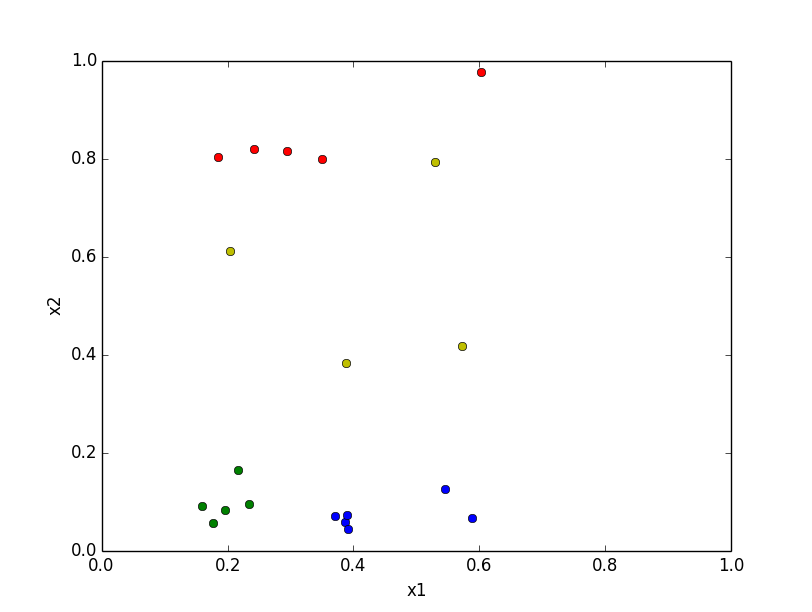
\includegraphics[width=0.9\textwidth]{figures/mlp_classification_10000.png}
    \caption{Classification produced by the multi-layer perceptron after 10000 epochs}
    \label{fig:mlp_classification_10000}
\end{figure}

\todo{Add the classification evolution for the decision tree ensemble}

\subsection{Learning curve}

The learning curve image for the neural network is shown in Figure~\ref{fig:mlp_learning_curve}.

\begin{figure}[p]
    \centering
    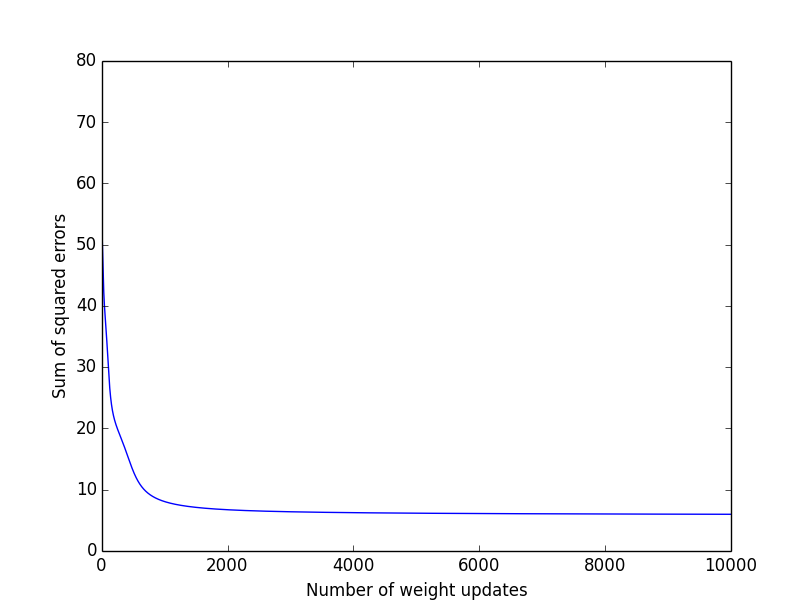
\includegraphics[width=0.9\textwidth]{figures/mlp_learning_curve.png}
    \caption{Learning curve for the multi-layer perceptron}
    \label{fig:mlp_learning_curve}
\end{figure}

%% And the learning curve image for the decision tree ensemble is shown in Figure~\ref{fig:tree_learning_curve}.

%% \begin{figure}[p]
%%     \centering
%%     \includegraphics[width=0.9\textwidth]{figures/tree_learning_curve.png}
%%     \caption{Learning curve for the decision tree ensemble}
%%     \label{fig:tree_learning_curve}
%% \end{figure}

\todo{Add the decision tree ensemble learning curve}

\section{Discussion}

With the data from the Section~\ref{sec:results}, we can see that the multi-layer perceptron correctly classified all the samples from the test data after 1000 epochs.
The learning curve shows us that the multi-layer perceptron is learning very quickly during the first updates, and then reach a plateau around the 2000 epochs.
We can see that first the multi-layer perceptron classifies all the samples as scraps. Then, after 10 epochs, all the samples are classified as rings. After 100 epochs, the majority of samples are correctly classified, however the class boundaries are still approximate. This is why the recognition rate is only 0.65. Finally, after 1000 epochs, the class boudaries are correct.

\todo{Describe the process for decision tree ensemble}

\todo{Compare the two methods}

\end{document}
